% !TEX root = ../IS.tex
\chapter{Extensive Form Games}
\section{Basics of Game Theory}
Frequently used, and originally explored in economic contexts, game theory is the study of interactions between decision-makers. Antoine Cournot attempted to explain the decisions of duopolies (markets with only two sellers producing a product) in 1838 using the concept of strategic behavior \cite{webs14}. In this case, strategic behavior refers to scenarios where one person's decisions both affect and are affected by the decisions of other persons. Cournot later influenced Joseph Bertrand's 1883 work, which examined strategic decisions in product pricing. These early efforts were limited by standard economic methodologies; it wasn't until John von Neumann's 1928 proof of the minimax theorem and his later collaboration with economist Oskar Morgenstern that the modern field of game theory began \cite{webs14}. The strategies involved with game theory are used to explain collusion and subsequent breakdown of oligopolies like OPEC, and the symbiosis between sharks and pilot fish.\\

As we begin our study of game theory, it is important to precisely define what games are.
\begin{define}
  A game is a description of a strategic interaction which constrains the actions a player can perform and the interests of players, but does not describe specifically which actions are performed \cite{osbo94}.
\end{define}

\begin{exmp}
  Chess is a game. In chess, players have a set of pieces, each with their own type of movement and attack pattern. The most important piece is the King, which can move and capture one space in any direction. However, if the King is under threat (i.e. an opponent's piece can capture the King on the next turn), then the King is considered to be in ``check.'' If the King is in check, cannot leave check, and no piece can capture or block the threatening piece, the King is in checkmate and the game ends.
\end{exmp}

For example, chess fits the definition of a game. The player's actions are constrained by the rules of the game and how each individual piece can move. The interest of the player is to checkmate the other player's king. However, the game does not specify that certain moves must be played.

Game theory involves the techniques used to analyze and determine solutions, strategies, and outcomes for various games \cite{osbo94}.
\begin{define}
  A solution of a game is the description of outcomes which may arise from the game \cite{osbo94}.
\end{define}

For the chess example, a single outcome of the game would be the sequence of actions which lead from the starting position of the game to a checkmate. The solution of chess is thus the collection of all sequences going from start to checkmate.\\

There are several types of solutions used in game theory, each being more useful in some games than in others \cite{osbo94}. Three solutions - Nash equilibrium, mixed strategies, and subgame equilibria - will be discussed later in this chapter.\\

It is assumed that players in these games are both \textit{rational} - they pursue well-defined objectives, generally in their own self-interest - and \textit{strategic} - they take the knowledge and behavior of other decision-makers into account \cite{osbo94}. With these assumptions, each decision made by a player is deliberate and involves optimization of some sort. Players consider their actions and the consequences thereof, and choose actions that best fit their preferences \cite{osbo94}. Returning to the chess example, players pursue their goal of checkmating the opponent's King, and they must plan ahead and predict what their opponent might do.\\

The preferences of these players are represented using a utility function. In game theory, \textit{utility} is the quantitative measure of a choice's value; this could be a monetary value or it could be expressed in terms of the happiness, measured with some metric, a player gains from that outcome, depending on the structure of the ``game''. A highly desired outcome for a player will have a higher utility than an undesirable outcome. In many games, the desired outcome for each player stands in diametric opposition to the desires of other players, referred to as a \textit{strictly competitive game} \cite{osbo94}. One type of strictly competitive game is a \textit{zero-sum game}.
\begin{define}
  A game is ``zero-sum'' if an action made by one player increases their utility by an amount equal to the loss in utility for the second player from that same action. Specifically, for an action $a$ and utility functions $u_1$ for player 1 and $u_2$ for player 2, $u_1(a)+u_2(a)=0$. Zero-sum games can only have two players \cite{shoh09}.
\end{define}

In a zero-sum game, every action which changes utility affects both players in the game. For every loss in utility, the other player gains an equal amount. Zero-sum games are a subset of \textit{constant-sum} games. In contrast with zero-sum, a constant-sum game will have an action $a$ where $u_1(a)+u_2(a)$ is equal to a constant $c$ \cite{shoh09}.

\begin{exmp}
  The card game War is a zero-sum game. In War, two players play the top card of their deck simultaneously. Whoever played the higher value card takes both cards and places them at the bottom of their deck. In the event of a tie, both players play two cards face-down and a third card face-up. The winner of this exchange takes all cards in play. The utility of each card can be measured by its face value, and the utility of each player is equal to the sum of the utility of all cards in their deck. Suppose that there is a round where Player 1 plays a 10 and Player 2 plays a Queen. Player 2 takes the 10, gaining 10 utility points while Player 1 loses those same 10 points. Let $u_1(a)$ represent the utility for player 1 of an interaction $a$ and $u_2(a)$ represent the utility for player 2 of an interaction $a$. Thus, if player 1 plays an 8 and player 2 plays a 4, player 1 will keep the 8 and take the 4. The utility $u_1((8, 4))=4$ since player 1 gained a 4 and $u_2((8, 4))=-4$ since player 2 lost a 4. Thus, $u_1(a)+u_2(a)=4-4=0$. This holds after every play in the game, so War is a zero-sum game.
\end{exmp}

In comparison, a non-zero-sum game does not have an equal exchange of utility. Interactions between players are unequal. One player may gain five utility points while another player loses three utility points, or one player may gain utility with no effect on other players.

\begin{exmp}
  Golf is not a zero-sum game. Suppose two players are competing on the same course for the best score. In golf, players are scored by the number of strokes it takes to reach each hole, with lower scores being more valuable than higher scores. If Player 1 takes two strokes on a particular hole, this only affects Player 1's score/utility; Player 2's utility is unaffected.
\end{exmp}

When games can be expressed in what is known as the \textit{normal form}, this zero-sum quality affects the strategies and solutions of these games.

\section{Normal Form Games}
In the vast majority of human choices, a person will attempt to maximize their utility function; they will perform actions that benefit themselves. When there are two or more agents trying to maximize their utility, the interactions and choices between these agents, or players, become more and more complex. These interactions can be studied with game theory using the \textit{normal} or \textit{strategic} form.
\begin{define}
  A finite normal-form game is a tuple $(N, A, u)$ where:
  \begin{itemize}
  \item $N$ is a finite set of $n$ players, indexed by $i$
  \item $A=A_1\times\cdots\times A_n$, where $A_i$ is a finite set of actions available to player $i$. Each vector $a=(a_1,\cdots ,a_n)\in A$ is called an action profile.
    \item $u=(u_1,\cdots ,u_n)$ where $u_i : A \mapsto\mathbb{R}$ is a real-valued utility function for player $i$. \cite{shoh09}
\end{itemize}
\end{define}

In an arbitrary normal-form game, there are $n$ different players contained in the set $N$, where $n$ is a positive integer. For each of these players, there is also a finite set of actions that they can take. Player $N_i$ will have the action set $A_i$. The complete action set $A$ is determined by the Cartesian product of the action sets of each player. Within $A$, a vector $a$ is the action profile; an action profile, or outcome, represents the choice that each player makes \cite{osbo94}. The collection of mappings $u$ gives each action profile a particular value; these values determine which outcome is preferred by a player. In normal-form games, players are utility-maximizing agents; they will gravitate towards action profiles that give them higher utility. An example of a normal-form game can be seen in the quintessential ``Prisoner's Dilemma'' example.\\

\begin{exmp}
  Two criminals are arrested in conjunction with two different crimes. The two are interviewed separately by the police. While in custody, each prisoner has a choice: they can either cooperate with their accomplice, or defect and testify to the police. Without a confession, the police only have enough evidence to convict them on the lesser of the two crimes, which has a sentence of 1 year in prison. If the police can get a confession, they will be able to convict for the greater crime, which has a 3 year sentence. If one prisoner defects, the police are prepared to drop their charges, and they will get no prison time while their accomplice gets the full 4 year total. If both prisoners defect they must both serve time; however, the judge will reward their cooperation with only a 3 year sentence. If both prisoners cooperate with each other (i.e. neither one confesses to the police), then they will both be convicted for the lesser crime and serve the 1 year sentence. The decisions in this game are expressed in a 2x2 matrix, with one player's choices represented in the columns and the other player's choices represented in the rows of said matrix.

\begin{figure}[H]
  \centering
  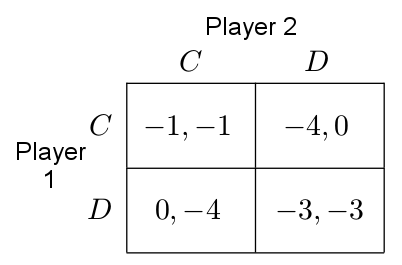
\includegraphics[width=7cm]{figures/ExampleGrid.png}
  \caption{The Prisoner's Dilemma, represented in a normal form matrix \cite{shoh09}.}
  \label{fig:prisoner}
\end{figure}
\end{exmp}

In Figure \ref{fig:prisoner}, the column labeled \textit{C} represents prisoner 2 cooperating with their partner, while the column labeled \textit{D} represents prisoner 2 defecting, telling the police that their partner is guilty. The rows \textit{C} and \textit{D} represent the same choices for prisoner 1. For this game, $A_i$ would be the set $\{C, D\}$, as those are the two choices that each prisoner can make. Thus, $A=A_1\times A_2 = \{(C, C), (C, D), (D, C), (D, D)\}$, or all four possible outcomes for this game. An action profile $a$ in this game would then be any of the ordered pairs in $A$; $(C,D)$, for instance, is an action profile. The ordered pairs within the matrix represent the values of each player's respective utility function in that outcome. In this case, their utility is the number of years in jail to which a player is sentenced. Since the players do not want to spend any time in prison, these utility values are negative; outcomes with less prison time have higher utility. The mapping functions in $u$ correspond to the leniency of the courts; unfortunately, the quantitative functions in $u$ that the courts use in this example are unknown, and only the values at these specific points are known. When both prisoners cooperate, they both get one year in prison; their sentence is lighter without their confession. If only one prisoner confesses, that player gets off with no time in prison, while the other player gets four years in jail. If both prisoners rat out their partner for committing the crime, both prisoners get three years in prison.\\

The prisoner's dilemma is not a zero-sum game. Supposing prisoner 1 chooses to defect ($D$), prisoner 2 could increase their utility from $-4$ to $-3$ by also defecting - a $+1$ change in utility for prisoner 2, but a $-3$ change in utility for prisoner 1.\\

From the perspective of an individual player, they must consider their options before proceeding. In considering their options, the best strategy can be determined using a game theory solution. In this example, the best strategy of a player would be trivial if that player also knew which strategies the other player(s) were adopting \cite{shoh09}. This would be a \textit{pure strategy} option, where the player selects a single action and always that action. The other option is for a player to create a \textit{mixed strategy} profile by introducing randomness into their own choice.

\begin{define}
  Let $(N,A,u)$ be a normal-form game, and for any set $X$ let $\Pi(X)$ be the set of all probability distributions over $X$. The set of mixed strategies for player $i$ is $S_i = \Pi(A_i)$, and the probability an action $a_x\in A_i$ will be played is denoted $s_i(a_x)$. A mixed-strategy profile is the Cartesian product of individual strategy sets $S_1\times\cdots\times S_n$ \cite{shoh09}.
\end{define}

For an example of both pure and mixed strategies, consider a game where one player offers the other a choice of two different toys.

\begin{exmp}
  There are two players and two presents containing toys. One player is designated the offering player, and the other player is designated the choosing player. The choosing player wants one of the toys, but not the other. The offering player picks which box to place each toy in, and the choosing player selects which present they want to open.
\end{exmp}

Suppose that the toys are placed in transparent boxes, and thus the contents of the boxes are not hidden. The offering player places each toy in a box, and the choosing player picks whichever toy gives them the most utility. In this case, the decision made by the offering player is virtually meaningless. It does not matter whether the toy desired by the choosing player is in box a or box b, since they can see which transparent box contains the toy they want. In this case, both the offering player and the choosing player use a pure strategy. Suppose instead that the toys are inside gift boxes - one red, one green. Once again, the offering player uses pure strategy to decide in which box to place each toy; they make a choice at the beginning of the game and stick with that choice. But, since the choosing player does not know which box contains their desired toy, they have a 50-50 chance of picking the toy they want. Thus, any pure strategy they might formulate (such as always picking the red box) will not be guaranteed to maximize the choosing player's utility. Thus, since it is unclear which decision is best, a mixed strategy is more appropriate. A pure strategy is a special case of mixed strategy, where the probability $s_i(a_x)=1$ for a particular value of $i$ and $s_i(a_k)=0 \forall a_k\in A_i, a_k \neq a_x$. With the mixed strategies determined, the players can find their \textit{best response} to a mixed-strategy profile.

\begin{define}
  A best response for player $i$ is a mixed strategy $s_i^*$. Let $S$ be the mixed-strategy profile for a normal-form game, and $s_{-i}$ be the set of strategy profiles disjoint from player $i$'s strategy profile $s_i$. The best response $s_i^*\in S_i$, such that $u_i(s_i^*,s_{-i}) \ge u_i(s_i, s_{-i})$ for all strategies $s_i\in S_i$ \cite{shoh09}.
\end{define}

In two-player games, like the toy choosing game, finding $s_{-i}$ is simple: if $i=1$, then $s_{-i}=s_2$, the strategy profile for player 2. In a three-player game with $i=1$, $s_{-i}$ would be $\{s_2, s_3\}$, the set containing player 2's strategy and player 3's strategy. For player $i$ to determine their best response, they must find a mixed strategy which maximizes utility against $s_{-i}$. In rare cases, this mixed strategy will actually be a unique pure strategy. Most of the time, there will be an infinite number of best responses with two or more actions in $s_i$ \cite{shoh09}. These actions must have the same value to the player, or else that player would want to minimize the probability of one such action. And therefore, since neither option is preferred over another, every possible combination of probabilities for actions in $s_i$ is a best response.\\

For the toy choosing game, the mixed-strategy profile is the Cartesian product of player 1 and player 2's strategy sets. To better illustrate the mixed-strategy profile, assume Player 1, the player offering the gifts, chooses to put the desired toy in box a or b by flipping a coin, rather than by pure strategy. Player 1's mixed-strategy set $S_1$ is therefore $\{.5a_1, .5b_1\}$. Player 2, the selecting player, chooses either box a or box b. Thus, player 2's mixed-strategy $S_2$ is $\{.5a_2, .5b_2\}$. The mixed-strategy profile for the entire game is therefore $\{(.5a_1, .5a_2), (.5a_1, .5b_2), (.5b_1, .5a_2), (.5b_1, .5b_2)\}$. In this example game, $S_1$ and $S_2$ are both a best response. Player 1 has no preference for either box a or box b; Player 2 does not know which box they prefer, and treats both equally.\\

Without knowing the strategy of other players, the most an agent can do is choose a strategy that is better than other strategies in all possible scenarios. This is known as the Nash equilibrium.

\begin{define}
  A strategy profile $s=(s_1,\dots ,s_n)$ is a Nash equilibrium if, for all agents i, $s_i$ is a best response to $s_{-i}$ \cite{shoh09}.
\end{define}

To find the Nash equilibrium for a player in the prisoner's dilemma example, the action of the other player is assumed to be a constant, pure strategy. So, while determining player 1's Nash equilibrium, we first assume that player 2 always cooperates with player 1. This assumption limits player 1's decision to a single column in the normal form.
\begin{figure}[H]
  \centering
  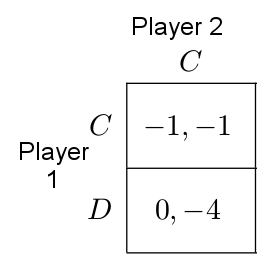
\includegraphics[width=5cm]{figures/ExamplePartialCol1.png}
  \caption{Player 1's best response in the Prisoner's Dilemma, assuming Player 2 cooperates with Player 1.}
  \label{fig:NashCol1}
\end{figure}

In Figure \ref{fig:NashCol1}, it is trivial to find the utility-maximizing strategy. In this case, the best response to player 2's cooperation is for player 1 to defect and accuse their partner: 1 year in prison by cooperating or no time in prison by defecting.\\

\begin{figure}[H]
  \centering
  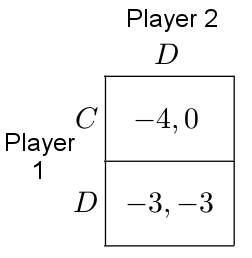
\includegraphics[width=5cm]{figures/ExamplePartialCol2.png}
  \caption{Player 1's best response in the Prisoner's Dilemma, assuming Player 2 will defect against Player 1.}
  \label{fig:NashCol2}
\end{figure}
Next, we assume that player 2 always defects. In Figure \ref{fig:NashCol2}, it is again trivial to find the utility-maximizing strategy for player 1. Assuming player 2 will defect to the police, player 1's best response is to defect as well: 3 years in prison by defecting or 4 years in prison by cooperating. So, for all of player 2's possible strategies, player 1's best response is to defect.\\

Using the same process for player 2, we first assume that player 1 uses pure strategy, and that their pure strategy is to cooperate with player 2.
\begin{figure}[H]
  \centering
  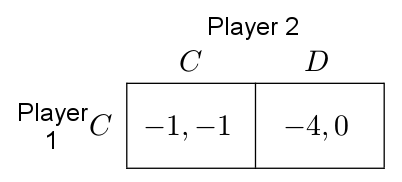
\includegraphics[width=7cm]{figures/ExamplePartialRow1.png}
  \caption{Player 2's best response in the Prisoner's Dilemma, assuming Player 1 will cooperate with Player 2.}
  \label{fig:NashRow1}
\end{figure}

In Figure \ref{fig:NashRow1}, it is trivial to find the utility-maximizing strategy. In this case, the best response to player 1's cooperation is for player 2 to defect and accuse their partner: 1 year in prison by cooperating or no time in prison by defecting.\\

\begin{figure}[H]
  \centering
  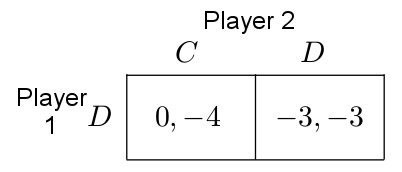
\includegraphics[width=7cm]{figures/ExamplePartialRow2.png}
  \caption{Player 1's best response in the Prisoner's Dilemma, assuming Player 2 will defect against Player 1.}
  \label{fig:NashRow2}
\end{figure}
Next, we assume that player 2 always defects. In Figure \ref{fig:NashRow2}, it is again trivial to find the utility-maximizing strategy for player 1. Assuming player 2 will defect to the police, player 1's best response is to defect as well: 3 years in prison by defecting or 4 years in prison by cooperating.\\

\begin{figure}[H]
  \centering
  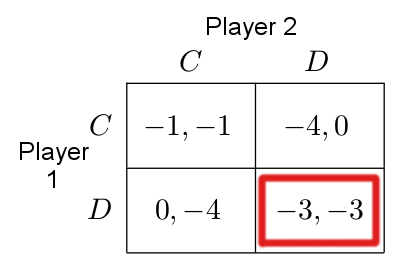
\includegraphics[width=7cm]{figures/ExampleNashEquilibrium.png}
  \caption{The Nash Equilibrium of the Prisoner's Dilemma: Both prisoners defect and both are sentenced to three years in prison.}
  \label{fig:NashEquil}
\end{figure}

So, for all of player 2's possible strategies, player 1's best response is to defect. Thus, the Nash equilibrium is that both prisoners will defect and get 3 years in prison, as seen in Figure \ref{fig:NashEquil}. A more robust proof of the Nash equilibrium for the Prisoner's Dilemma is shown below.



%% ------------------------------------------------
%% Proof of Nash Equilibrium for Prisoner's Dilemma
%% ------------------------------------------------
\begin{thm}
  Assume a normal form game $G = (N, A, u)$, $N=\{n_1, n_2\}$, and $A=\{A_1\times A_2\} = \{c_1, d_1\}\times\{c_2, d_2\}$. If the set of utility functions $u = \{u_1=(c_1, c_2)\mapsto -1, (c_1, d_2)\mapsto -4, (d_1, c_2)\mapsto 0, (d_1, d_2)\mapsto -3\}, u_2=(c_1, c_2)\mapsto -1, (c_1, d_2)\mapsto 0, (d_1, c_2)\mapsto -4, (d_1, d_2)\mapsto -3$, then the Nash equilibrium of $G$ is the strategy profile $(d_1, d_2)$, where $d_1$ is the choice for player 1 to defect and $d_2$ is the choice for player 2 to defect.
\end{thm}
\begin{proof}
  Let $G=(N, A, u)$ be a normal-form game. $N = \{n_1, n_2\}$ is the set of players in the game. $A=A_1\times A_2$ is the set of actions in the game, where $A_1=\{c_1, d_1\}$ is the set of actions available to player 1, and $A_2=\{c_2, d_2\}$ is the set of actions available to player 2. Therefore, $A=\{(c_1, c_2), (c_1, d_2), (d_1, c_2), (d_1, d_2)\}$. The utility function $u=(u_1, u_2)$. $u_1=(c_1, c_2)\mapsto -1, (c_1, d_2)\mapsto -4, (d_1, c_2)\mapsto 0, (d_1, d_2)\mapsto -3$, and $u_2=(c_1, c_2)\mapsto -1, (c_1, d_2)\mapsto 0, (d_1, c_2)\mapsto -4, (d_1, d_2)\mapsto -3$.\\

  Let $s^*_1$ be a mixed strategy for $n_1$ where $n_1$ chooses action $d_1$ with a probability of 1. Since there are only two players, the set of strategy profiles disjoint from $s_1$ is the same as $s_2$, the set of strategy profiles for $n_2$. Thus, $n_1$ has $s^*_1$ as a best response to $s_2$ if $u_1(s^*_1, s_2)\ge u_1(s_i, s_2)$ for all possible actions $s_i\in A_1$ and all strategies in $s_2$.\\
  
  $u_1(d_1, c_2)\ge u_1(c_1, c_2) \Rightarrow 0\ge -1$\\
  
  $u_1(d_1, c_2)\ge u_1(d_1, c_2) \Rightarrow 0\ge 0$\\

  $u_1(d_1, d_2)\ge u_1(c_1, d_2) \Rightarrow -3\ge -4$\\

  $u_1(d_1, d_2)\ge u_1(d_1, d_2) \Rightarrow -3\ge -3$\\

  $s^*_1$ is greater than or equal to all possible actions in $A_1$ and for all strategies in $s_2$. Thus, $s^*_1=d_1$ is the best response for player $n_1$.\\

  Let $s^*_2$ be a mixed strategy for $n_2$ where $n_2$ chooses action $d_2$ with a probability of 1. Since there are only two players, the set of strategy profiles disjoint from $s_2$ is the same as $s_1$, the set of strategy profiles for $n_1$. Thus, $n_2$ has $s^*_2$ as a best response to $s_1$ if $u_2(s^*_2, s_1)\ge u_2(s_i, s_1)$ for all possible actions $s_i\in A_2$ and all strategies in $s_1$.\\
  
  $u_1(c_1, d_2)\ge u_1(c_1, c_2) \Rightarrow 0\ge -1$\\

  $u_1(c_1, d_2)\ge u_1(c_1, d_2) \Rightarrow 0\ge 0$\\

  $u_1(d_1, d_2)\ge u_1(d_1, c_2) \Rightarrow -3\ge -4$\\

  $u_1(d_1, d_2)\ge u_1(d_1, d_2) \Rightarrow -3\ge -3$\\

  $s^*_2$ is greater than or equal to all possible actions in $A_2$ and for all strategies in $s_1$. Thus, $s^*_2=d_2$ is the best response for player $n_1$.\\

  A strategy set $(s_1,\dots ,s_n)$ is a Nash equilibrium if $s_i$ is the best response for all players $i$. Therefore, the strategy profile $(d_1, d_2)$ is a Nash equilibrium for the game $G$, the Prisoner's Dilemma.
\end{proof}
Using the definition of a best response, it can be shown that choosing to defect is the best response in the prisoner's dilemma for both player 1 and player 2. The utility payout of these responses is -3 for both players.

Not all games have a Nash equilibrium; take the normal-form representation of rock-paper-scissors, for instance.

\begin{exmp}
  In Rock-Paper-Scissors, two players choose a hand sign at the same time. If both play the same sign, the round is a draw. If two different signs are played, a winner is determined using the following rules: rock beats scissors, scissors beat paper, and paper beats rock. Let the players 1 and 2 have utility functions which award players 1 point for winning the game, -1 point for losing the game, and 0 points for a draw. Notice that these values create a zero-sum game; a win for Player 1 comes with a loss for Player 2. We position Player 1 on the left side of the matrix, and Player 2 on the top of the matrix.
  \begin{figure}[H]
    \centering
    \begin{tabular}{r r | c | c | c |}
      &\multicolumn{1}{c}{}&\multicolumn{1}{c}{}&\multicolumn{1}{c}{Player 2}&\multicolumn{1}{c}{}\\
      Rock-Paper-Scissors &\multicolumn{1}{c}{}&\multicolumn{1}{c}{Rock}&\multicolumn{1}{c}{Paper}&\multicolumn{1}{c}{Scissors} \\ \cline{3-5}
      & Rock & (0, 0) & (-1, 1) & (1, -1) \\ \cline{3-5}
      Player 1 & Paper & (1, -1) & (0, 0) & (-1, 1) \\ \cline{3-5}
      & Scissors & (-1, 1) & (1, -1) & (0, 0) \\ \cline{3-5}
    \end{tabular}
    \caption{The normal-form representation of the game Rock-Paper-Scissors}
    \label{fig:RPS}
  \end{figure}
\end{exmp}

Every row and every column in Figure \ref{fig:RPS} has the same three results, and none of the choices is a winning strategy for more than one situation. Rock may beat Scissors, but it loses to Paper. If the Nash equilibrium of Player 1 is investigated, each possible action by Player 2 results in a different best response for Player 1. For every situation where Player 1's choice provides the most utility, there exists another, equally-likely situation where the same choice would provide the least utility (in this case, negative utility) and a third equally likely situation where that choice provides no utility. Therefore, there can be no Nash equilibrium.\\

\subsection{Non-Simultaneous Games}
It is important to recognize in these two examples that both players are making their choice simultaneously. Games without simultaneous actions are not so easily expressed in normal form. For example, take a game of tic-tac-toe. For simplicity, assume that the game is played with a 2x2 board instead of a 3x3 board. Assume the utility function awards players 1 point for winning the game, -1 point for losing the game, and 0 points for a draw. Let UL be a piece in the upper left square, UR the upper right square, LL the lower left square, and LR the lower right square. We position Player 1 on the left side of the matrix, and Player 2 on the top of the matrix. Assume Player 1 has the first turn.\\
\begin{figure}[H]
  \centering
  \begin{tabular}{r r | c | c | c | c |}
    &\multicolumn{1}{c}{}&\multicolumn{1}{c}{}&\multicolumn{1}{c}{Player 2}&\multicolumn{1}{c}{}\\
    \multicolumn{1}{c}{2x2 tic-tac-toe}&\multicolumn{1}{c}{}&\multicolumn{1}{c}{UL}&
    \multicolumn{1}{c}{UR}&\multicolumn{1}{c}{LL}&\multicolumn{1}{c}{LR}\\ \cline{3-6}
    & UL & x & (0, 0) & (0, 0) & (0, 0) \\ \cline{3-6}
    Player 1 & UR & (0, 0) & x & (0, 0) & (0, 0) \\ \cline{3-6}
    & LL & (0, 0) & (0, 0) & x & (0, 0) \\ \cline{3-6}
    & LR & (0, 0) & (0, 0) & (0, 0) & x \\ \cline{3-6}
  \end{tabular}
  \caption{The first two moves of a tic-tac-toe variant using a 2x2 game board.}
  \label{fig:2x2TTT}
\end{figure}

Figure \ref{fig:2x2TTT} shows the normal form for the first two moves of this game. Since each player has only placed a single piece, neither one has won yet; thus, the utility for each space is (0,0). There are four spaces in the matrix marked with an 'x'. These spaces are infeasible; it is against the rules for someone to play on the same square as someone else. Both players have made their first move, and it is Player 1's turn once again.\\
\begin{figure}[H]
  \centering
  \begin{tabular}{r r | c | c | c | c |}
    &\multicolumn{1}{c}{}&\multicolumn{1}{c}{}&\multicolumn{1}{c}{Player 2}&\multicolumn{1}{c}{}\\
    \multicolumn{1}{c}{2x2 tic-tac-toe}&\multicolumn{1}{c}{}&\multicolumn{1}{c}{UL}&
    \multicolumn{1}{c}{UR}&\multicolumn{1}{c}{LL}&\multicolumn{1}{c}{LR}\\ \cline{3-6}
    & (UL, UR) & x & x & (1, -1) & (1, -1) \\ \cline{3-6}
    & (UL, LL) & x & (1, -1) & x & (1, -1) \\ \cline{3-6}
    & (UL, LR) & x & (1, -1) & (1, -1) & x \\ \cline{3-6}
    & (UR, UL) & x & x & (1, -1) & (1, -1) \\ \cline{3-6}
    & (UR, LL) & (1, -1) & x & x & (1, -1) \\ \cline{3-6}
    Player 1 & (UR, LR) & (1, -1) & x & (1, -1) & x \\ \cline{3-6}
    & (LL, UL) & x & (1, -1) & x & (1, -1) \\ \cline{3-6}
    & (LL, UR) & (1, -1) & x & x & (1, -1) \\ \cline{3-6}
    & (LL, LR) & (1, -1) & (1, -1) & x & x \\ \cline{3-6}
    & (LR, UL) & x & (1, -1) & (1, -1) & x \\ \cline{3-6}
    & (LR, UR) & (1, -1) & x & (1, -1) & x \\ \cline{3-6}
    & (LR, LL) & (1, -1) & (1, -1) & x & x \\ \cline{3-6}
  \end{tabular}
  \caption{The full normal form representation of a 2x2 tic-tac-toe variant}
  \label{fig:full2x2TTT}
\end{figure}

By nature of this compressed game board, the first player to place their piece (in this case, player 1) cannot lose; all legal moves lead to victory. But even in this simplified game, the normal form in Figure \ref{fig:full2x2TTT} quickly becomes convoluted and cluttered. While the infeasible actions are fairly self-evident in Figure \ref{fig:2x2TTT}, illegal moves are less obvious in Figure \ref{fig:full2x2TTT}.
\begin{figure}[H]
  \centering
  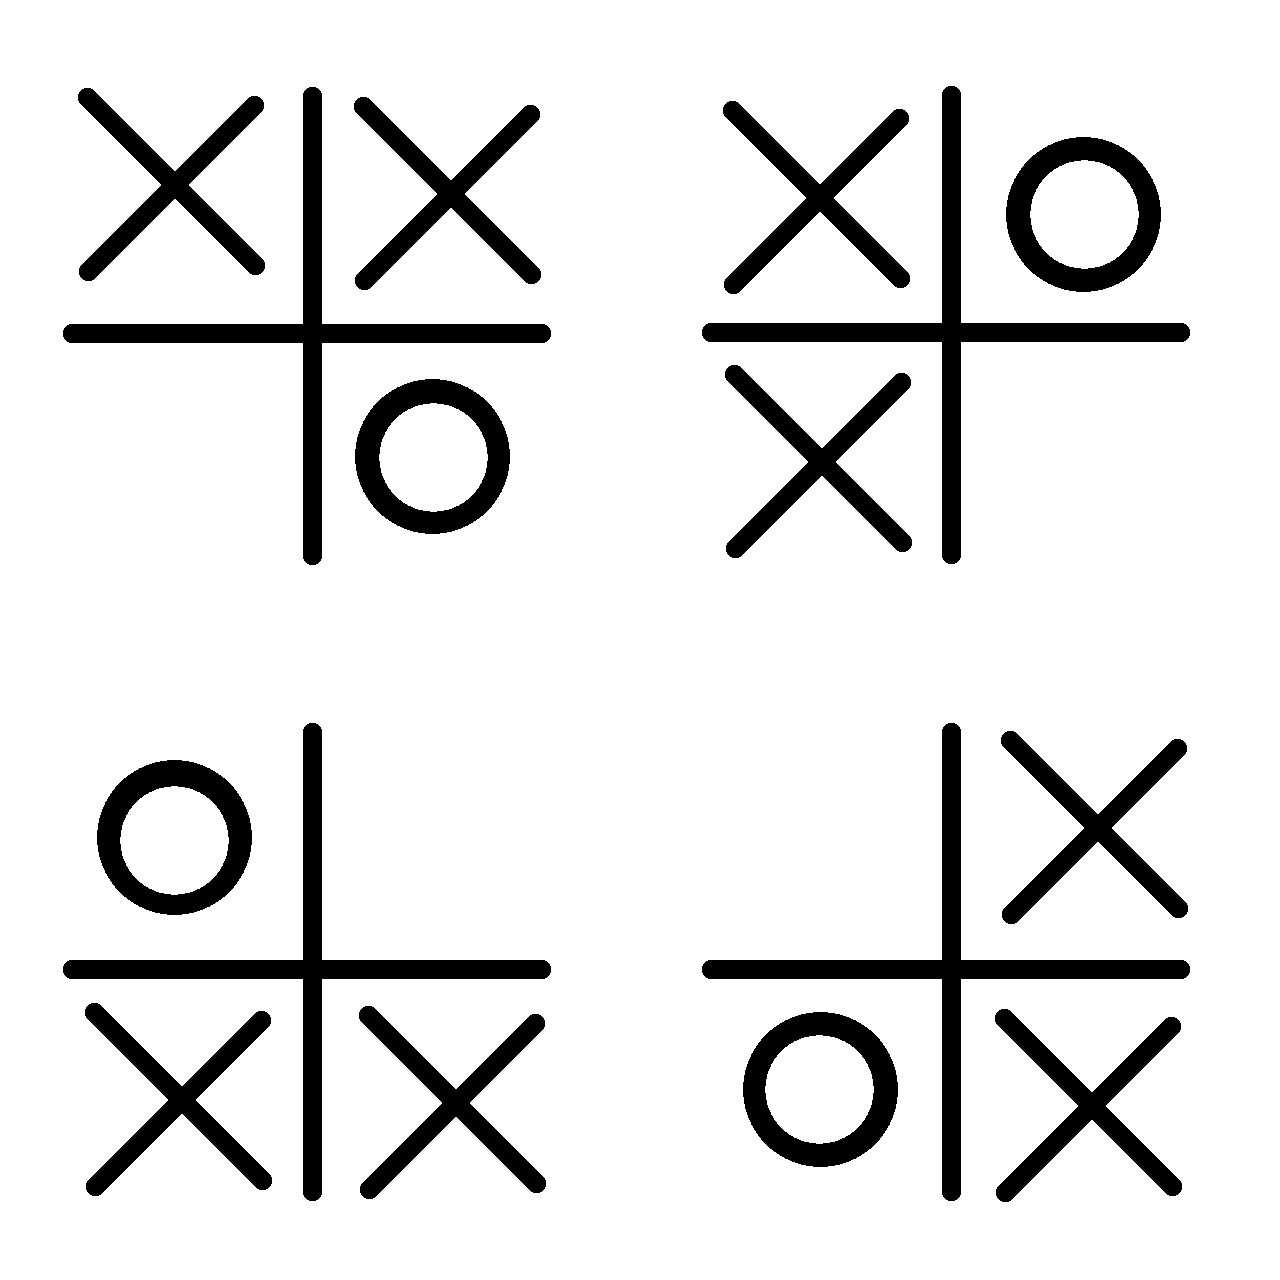
\includegraphics[width=6cm]{figures/TTTRotation.png}
  \caption{Rotational symmetry in a 2x2 tic-tac-toe game}
  \label{fig:2x2TTTRotation}
\end{figure}
There are also repeated game configurations: the outcome \{(UL, UR), (LR)\} is rotationally symmetrical to \{(LL, UL), (UR)\}, \{(LR, LL), (UL)\}, and \{(UR, LR), (LL)\}, as is evident in Figure \ref{fig:2x2TTTRotation}. Furthermore, the game \{(UL, UR), (LR)\} is identical to \{(UR, UL), (LR)\}. With so many extraneous spaces in the normal-form representation, it is no longer sufficient to represent player choices for games with sequential actions. Instead, these games are better represented in extensive-form trees.\\

\section{Extensive Form Trees}
In a turn-based, or an extensive-form game, players do not make simultaneous actions. This leads to larger variety in gameplay. A simultaneous game like Rock-Paper-Scissors relies on chance; tic-tac-toe relies on players anticipating the future choices their opponents will make. There are two types of extensive-form games: perfect-information and imperfect-information. In perfect-information games, all players know which turn of the game they are at, while imperfect-information games have turns that are indistinguishable from others based on information available to the player. For example, the card game Go Fish is an imperfect-information game: any individual guess is mostly indistinguishable from another. Even if player A determines that player B has no ``5's,'' for instance, that fact could change when player B draws another card. We will focus on perfect-information games.\\

These games are represented in graph-theoretic trees. Specifically, extensive-form games are represented with \textit{rooted trees}.
\begin{define}
  A rooted tree is a pair $(V, E)$, where $V$ (known as the vertex set) is a finite set and $E$ (known as the edge set) is a binary relation on $V$ \cite{corm09}. Elements of $V$ are referred to as vertices or nodes, and elements of $E$ are referred to as edges. Trees are acyclic, meaning that no cycles exist in the graph; there is no path which moves away from a node $a$ by edge $e$ and returns to $a$ by a different edge. Trees are connected, meaning every vertex in $V$ can be reached from all other vertices in $V$. One element $v\in V$ is denoted as the root.
\end{define}

These types of graphs are called trees due to the visualization in a tree-like diagram, showing the \textit{root} and \textit{children} (see Figure \ref{fig:sharingTree}).

\begin{define}
  A finite perfect information game in extensive form is a tuple $G = (N, A, H, Z, \chi, \rho, \sigma, u)$ where:
  \begin{itemize}
  \item $N$ is a set of n players;
  \item $A$ is a single set of actions;
  \item $H$ is a set of non-terminal, choice nodes;
  \item $Z$ is a set of terminal nodes, disjoint from $H$;
  \item $\chi: H\mapsto 2^A$ is the action function, mapping a set of possible actions to each choice node;
  \item $\rho: H\mapsto N$ is the player function, mapping to each non-terminal node a player who makes an action at said node;
  \item $\sigma: H\times A\mapsto H\bigcup Z$ is the successor function, mapping a choice node and an action to a new choice or terminal node. $\forall h_1, h_2\in H$ and $a_1, a_2\in A$, if $\sigma(h_1, a_1)=\sigma(h_2, a_2)$, then $h_1=h_2$ and $a_1=a_2$;
  \item $u=(u_1,...,u_n)$, where $u_i:Z\mapsto \mathbb{R}$ is a real-valued utility function for each player $i$ on a terminal node $Z$ \cite{shoh09}.
  \end{itemize}
\end{define}

As in the normal-form definition, there are $n$ players in the game, contained in the set $N$. $A$ is the set of all actions that could be performed in the course of the game. The set $H$ contains any and all choices or turns that do not end the game, while $Z$ contains all choices or turns that do end the game. The mapping function $\chi$ allocates the choices in $H$ a subset of possible actions from the set $A$, and the mapping function $\rho$ assigns these choices to the players who make them. $\sigma$ takes the actions assigned with $\chi$ and uses them to connect various nodes in $H$ and $Z$ together, creating the sequence of events in the game. Finally, $u$ contains utility functions for each player that determine their individual utility at each of the terminal nodes in $Z$. An example of the extensive-form tree can be seen in The Sharing Game.\\

\begin{exmp}
  In The Sharing Game, a variation of the toy-offering game in Example 2.2.2, two children receive two identical presents from their parents, both equally valuable to the children. Player 1 suggests one of three splits: Player 1 receives both presents, Player 2 receives both presents, or each player receives one present. Once the split has been suggested, Player 2 chooses to accept the split or not. If the split is declined, neither player receives any presents.

  \begin{figure}[H]
    \centering
    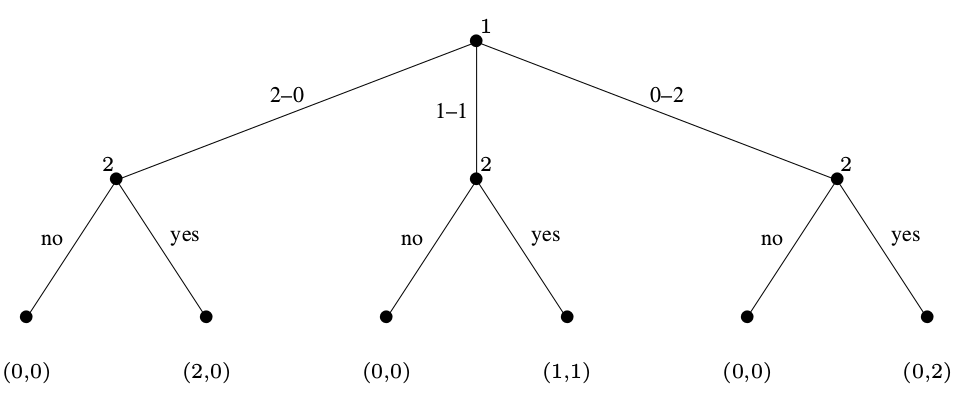
\includegraphics[width=10cm]{figures/ExampleTree.png}
    \caption{An extensive-form tree for The Sharing Game \cite{shoh09}}
    \label{fig:sharingTree}
  \end{figure}
\end{exmp}

Figure \ref{fig:sharingTree} shows six leaf nodes of this tree - the elements of the set $Z$ - while the other nodes are contained in $H$. The $H$ nodes are labeled either 1 or 2, denoting from the $\rho$ function which player is making the choice at that node. The $Z$ nodes each have a pair, denoting the utility each player will gain if the game ends in that particular way. The actions $A$ are denoted in the lines connecting the nodes together. In this game, the three actions from the root node are the methods of sharing 2 presents between 2 people. The second player, once the first player has distributed the presents in a particular way, chooses whether to accept the distribution or not.\\

To explore this definition, return to the game of 2x2 tic-tac-toe. Let $N=\{N_1, N_2\}$ be the set of players in the game. In this game, $A$ is the set of open spaces on which a player can place their symbol; for the first move of the game, $A$ is the set of 4 open spaces on the board, for the second move, $A$ is the set of the remaining 3 spaces. For a game of tic-tac-toe, $H$ contains configurations of the board where neither player has two in a row and there are still open squares on the board. $Z$, on the other hand, contains the board configurations where one player has two in a row or all spaces have been claimed. For tic-tac-toe, the $\chi$ function removes illegal actions from a node, which for tic-tac-toe would be playing on an occupied square. Thus, the $\chi$ function leaves the choice nodes at each successive turn with fewer and fewer available actions. Since there are only two players, the $\rho$ function alternates between players after each action.

\begin{figure}[H]
  \centering
  
\includegraphics[width=16cm]{figures/TTTExtTree.png}
  \caption{The extensive-form representation of a 2x2 tic-tac-toe game}
  \label{fig:2x2TTTExtForm}
\end{figure}

Figure \ref{fig:2x2TTTExtForm} shows the extensive-form version of the 2x2 tic-tac-toe variant in Figure \ref{fig:full2x2TTT}. In comparison to the normal-form representation, the extensive-form tree can convey the sequence and flow of the game more clearly. Since the $\chi$ function of an extensive-form game only maps possible actions, the tree does not have the same infeasible nodes as the normal-form representation. This tree has the same issues of rotational symmetry as in the normal form, but in this particular example, the four subtrees connected to the root are all rotationally symmetrical to each other.

\subsection{Equilibria in Extensive-Form}
Nash equilibria can be found in extensive-form games as well, and are defined the same as in normal-form games. However, a pure strategy in an extensive-form game requires the player's strategy to contain the decision at every choice node, even if that node is unreachable by other choices in said strategy.\\
\begin{define}
  Let $G = (N, A, H, Z, \chi, \rho, \sigma, u)$ be a perfect-information extensive-form game. The pure strategies of player $i$ consist of the Cartesian product $\Pi_{h\in H, \rho(h)=i}\chi(h)$ \cite{shoh09}.
\end{define}
Given a perfect-information game, a player's pure strategy is the set of choices mapped by $\chi$ from each of that player's choice nodes $h$. It is a complete specification of the choices that a player determines they should make \cite{shoh09}. Since the actions of all other players are known in an extensive-form game, it is not necessary to introduce probabilities to determine a Nash equilibrium. Instead, Nash equilibria can be found using backwards induction.

\begin{figure}[H]
  \centering
  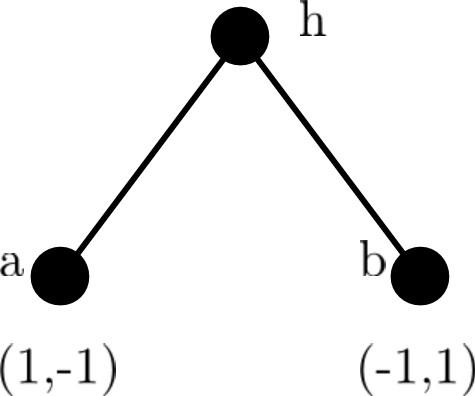
\includegraphics[width=4cm]{figures/ExampleBackwardInduction.png}
  \caption{A small extensive-form tree. The outcome is dependent on the player mapped by $\rho(h)$.}
  \label{fig:BackwardInduction}
\end{figure}

Backwards induction determines a dominant strategy for a particular game. This strategy works on the assumption that players act optimally, and will thus always choose a leaf node which maximizes their utility. Therefore, a decision node $n$ with a set of leaf nodes as its children is equivalent to the leaf which maximizes the utility of the deciding player. For example, examine the extensive-form tree for a two-player game in Figure \ref{fig:BackwardInduction}. with a root and two child nodes. Both of these children are leaf or terminal nodes. At the leaf node $a$, player 1 has positive utility while player 2 has negative utility; at leaf node $b$, player 2 has positive utility and player 1 has negative utility. Since both players are utility-maximizing agents, the choice of the outcome is determined by whichever player happens to be making the decision, as mapped by $\rho(h)$. Suppose that Figure \ref{fig:BackwardInduction} is a subtree in a larger game. Further suppose that, in this larger game, the subtree in Figure \ref{fig:BackwardInduction} always has player 1 making the choice at node $h$. Given this scenario, player 1 will always perform the action that gets them to node $a$. Thus, a tree where node $h$ is replaced by $a$, with $b$ being removed from the tree entirely, is equivalent to the current tree in Figure \ref{fig:BackwardInduction}. If the entire tree for a game is mapped out, then this process can be repeated all the way up to a root node; at that point, the outcome of the game can be determined before the game even begins. The pseudocode below describes the process of finding a subgame-perfect equilibrium from the bottom of an extensive tree upward.\\

\lstset{language=pseudocode, label={lst:BackwInd}, caption={The Backward Induction algorithm for extensive-form game trees \cite{shoh09}.}}
\begin{lstlisting}[language=pseudocode]
  Procedure BackwardInduction(node h)
  if(h in Z)
      return u(h)
      //If h is a leaf node, return the utility of that outcome
  end if
  for(a in %*$\chi$*(h))
      util_at_child = BackwardInduction(%*$\sigma(h, a)$*)
      //Recursively check each child of h
      if(util_at_child%*$_{\rho(h)}$* > best_util%*$_{\rho(h)}$*)
          best_util = util_at_child
          //best_util holds the node which maximizes the utility of player %*$\rho$*(h)
      end if
  end for
  return best_util
  end Procedure
\end{lstlisting}

The algorithm in Listing \ref{lst:BackwInd} has a base case at line 2, where $h$ is in the set of terminal nodes in $Z$, or the leaves of the extensive-form tree. At these leaves the game is over, and the utility of that outcome is returned by the algorithm. When the node in question is not a terminal node, the algorithm checks the utility of each of that node's children at line 6. Since the child nodes may have their own children, line 7 recursively checks each child and gets the utility of that node. In lines 9 and 10, the backwards induction algorithm determines which node provides the player at node $h$ (as determined by the mapping function $\rho$) the maximum amount of utility. This node is returned in line 14.\\

\begin{figure}[H]
  \centering
  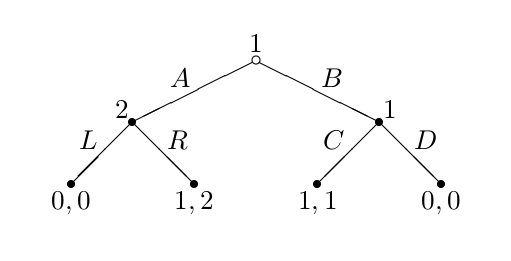
\includegraphics[width=8cm]{figures/NoBackward.png}
  \caption{An extensive-form game tree which cannot be completely solved with backward induction.}
  \label{fig:noBackward}
\end{figure}

Not all game trees can be reduced with the backwards induction algorithm. In Figure \ref{fig:noBackward}, two players play such a game.

\begin{exmp}
  Player 1 has a choice between $A$ and $B$ on their first turn. If Player 1 chooses $B$, then they make a second choice between $C$ and $D$. Player 2 only has one choice: if Player 1 chooses $A$, then Player 2 chooses between $L$ and $R$.
\end{exmp}
Using the backwards induction algorithm on the left subtree of Figure \ref{fig:noBackward}, we find that the outcome (1, 2) - the leaf node reached by the choices $\{A, R\}$ - is preferred by Player 2 to the outcome (0, 0) - the leaf node reached by the choices $\{A, L\}$. Thus, Player 2's choice node is replaced with the leaf node with utility (1, 2). On the right subtree in Figure \ref{fig:noBackward}, Player 1 makes a similar choice between (1, 1) - from the choices $\{B, C\}$ - and (0, 0) - from the choices $\{B, D\}$. Thus, the right child of the root is replaced with the leaf node with a utility value of (1, 1). Now, the algorithm can find the expected utility value of the root node. Since Player 1 is making the decision at the root, their choices have equal utility values: 1. Thus, Player 1 should have no preference to choosing $A$ or $B$. However, Player 2 does have a preference in this matter, but no way to influence Player 1's choice. Backwards induction is insufficient in this game to predict, with complete accuracy, whether the final outcome of the game will be (1,2) or (1,1).

\section{Other Games}
While normal-form and extensive-form games are the two largest categories of games, there are other types of games independent of the former two. One such type is \textit{repeated games} and \textit{stochastic games}.\\

Compared to the games previously discussed, referred to as \textit{one-shot games}, repeated games involve the same players playing the same game multiple times \cite{mail06}. Repeated games deal with the notion of trust, and what players expect their fellow players to do. After multiple iterations of the same game, players may start to predict their opponent's choices. However, these repetitions also encourage certain behaviors. For example, take the card game poker.
\begin{exmp}
  In poker, players are dealt a hand of playing cards and make bets on their hands; for instance, a player may bet \$100 that their hand has a higher rank than the hands of their opponents. These bets go into a communal pot, which is awarded at the end of the game. After a bet, the other players then have a chance to call the bet (adding in \$100 of their own to the bet), raising the bet (for instance, betting \$150 that their hand has the highest rank), or folding (exiting the game with no chance to regain the money in the pot). After a certain number of betting rounds, all players who have not folded show their hands, and the player with the highest ranking hand wins the money in the pot. The number of cards dealt, whether cards are dealt face-up or face-down, and the rank of various hands depend on the poker variant.
\end{exmp}

Suppose in the poker example that the same group of players play ten rounds against each other. After the first few rounds, players can infer some of the strategies employed by other players by earlier repetitions of the game. For instance, suppose a player always bluffs, pretending that they have a high-ranking hand even when they have a worthless hand. When this player, who we denote as player $A$, first bluffs in this manner, they may convince other players to fold. Thus, player $A$ may win some early rounds by deception. However, if in repeated games other players recognize player $A$'s strategy, they will become less susceptible to player $A$'s lies. In this way, the repeated nature of the game creates incentives fundamentally different from those of a one-shot game \cite{mail06}.\\

There is a repeated version of the Prisoner's Dilemma as well. As established in Figure \ref{fig:NashEquil}, the Nash equilibrium of the game is for both players to defect and to both serve three years in jail. This equilibrium comes about because players value the short-term goal of reaching a (0, -4) utility outcome \cite{osbo94} and both players are assumed to play optimally. However, it is possible that, without loss of generality, player 2 will not play optimally and choose to cooperate instead of defect as the Nash equilibrium would suggest. Since the original version of the Prisoner's Dilemma is a one-shot game, this scenario would greatly benefit player 1. However, in a repeated game, the defection strategy is no longer optimal.\\

In stochastic games, the actions taken by players has an effect on the \textit{environment} of the game \cite{sola15}. At each step of the game, play moves from position to position. These positions are determined by \textit{transition probabilities}, which both players in the game control \cite{shap53}. At any position of the game, each combination of choices for the two players has a probability greater than zero of ending the game and a probability of moving to another position of the game. For example, take the party game Twister.
\begin{exmp}
  In Twister, players contort themselves on a large playing mat. The mat has four columns of dots, with each column's dots in a different color. A neutral entity uses a spinner, which is split into quarters: right hand, left hand, right foot, and left foot. Each of these sections is further split into the four colors. When this neutral entity spins the spinner, players must perform the indicated action; for example, if the spinner lands on ``right foot red,'' all players must move their right foot onto a red dot. Players continue until they fall down, at which point they are out of the game.
\end{exmp}

At the starting position of the game, no players have any of their limbs on the playing mat. Suppose without loss of generality that the first turn is for players to move their right foot to a red dot. The probability of the game ending at this position will depend on which red dots players use. If players move their feet to distant red dots, so that their legs are spread far apart, it is more likely that the game will end than if players choose closer red dots. However, there is still the possibility that a player will slip and fall on the first step, even at the closest red dots.\\

Assume that play has continued further into the game, to an arbitrary position of limbs. The environment in Twister is dependant on the contortions into which players have put themselves. Thus, players have a preference to move themselves in ways which create more stable positions. Since there are a limited number of dots to which players can move, these positions get in the way of other players, and can cause them to lose their balance. Thus, players must find a metaphorical balance between keeping themselves stable and interferring with their opponents to be successful at the game.

\section{Conclusion}
Game theory provides a number of techniques and methods to find optimal strategies for games. These techniques can be applied to a wide variety of game types, including both games where players act simultaneously and games where players take turns acting. Game theory can also explain games where choices in one game affect choices in later iterations of the game, and games where a player's action affects the environment of the game.\\